 
\chapter{Konzept}
\label{sec:konzept}

\section{Vorgehensweise}
\label{sec:konzept:vorgehensweise}
Für die Umsetzung in diesem Projekt eigen sich der Apriori Algorithmus (oder eine Variante davon), welcher im ersten Schritt des \nameref{sec:recherche:dataminingtechniken:disziplinen:association} (\cref{sec:recherche:dataminingtechniken:disziplinen:association}) verwendet wird sowie die \nameref{sec:recherche:dataminingtechniken:disziplinen:clusteranalysis} (\cref{sec:recherche:dataminingtechniken:disziplinen:clusteranalysis}), welche in diesem Abschnitt weiter beschrieben werden.

\nameref{sec:recherche:dataminingtechniken:disziplinen:classification} (\cref{sec:recherche:dataminingtechniken:disziplinen:classification}) fällt weg, da damit bekannte Klassen zugeteilt werden welche in diesem Projekt jedoch nicht bekannt sind. Die \nameref{sec:recherche:dataminingtechniken:disziplinen:regression} (\cref{sec:recherche:dataminingtechniken:disziplinen:regression}) eignet sich nicht, da dadurch nur numerische Werte vorausgesagt werden können, in dieser Arbeit jedoch Klassen vergeben werden müssen. \nameref{sec:recherche:dataminingtechniken:disziplinen:collaborativefiltering} (\cref{sec:recherche:dataminingtechniken:disziplinen:collaborativefiltering}) versucht durch Kundenbewertungen ähnliche Objekte vorzuschlagen. Dies kann für einen Recommender eingesetzt werden, jedoch nicht für die Auffindung von häufigen Attributen.

%Die Umsetzung in diesem Projekt wird zweistufig durchgeführt. Als erstes gibt der User eine Abfrage ein, für welche anschliessend eine eine Liste von häufig auftretenden Attributen gesucht werden soll (siehe \cref{sec:einletung:ziel} \nameref{sec:einletung:ziel}). Die Abfrage schränkt dabei den Datenbestand ein. Dafür kann der erste Schritt des \nameref{sec:recherche:dataminingtechniken:disziplinen:association} (\cref{sec:recherche:dataminingtechniken:disziplinen:association}) eingesetzt werden. Für die Analyse der Restmenge eignet sich die \nameref{sec:recherche:dataminingtechniken:disziplinen:clusteranalysis} (\cref{sec:recherche:dataminingtechniken:disziplinen:clusteranalysis}), da zu Beginn die Klassen noch nicht bekannt sind. Dadurch fällt \nameref{sec:recherche:dataminingtechniken:disziplinen:classification} (\cref{sec:recherche:dataminingtechniken:disziplinen:classification}) weg. Die \nameref{sec:recherche:dataminingtechniken:disziplinen:regression} (\cref{sec:recherche:dataminingtechniken:disziplinen:regression}) eignet sich nicht, da dadurch nur numerische Werte vorausgesagt werden können, in dieser Arbeit jedoch Klassen vergeben werden müssen. \nameref{sec:recherche:dataminingtechniken:disziplinen:collaborativefiltering} (\cref{sec:recherche:dataminingtechniken:disziplinen:collaborativefiltering}) versucht durch Kundenbewertungen ähnliche Objekte vorzuschlagen. Dies kann für einen Recommender eingesetzt werden, jedoch nicht für die Auffindung von häufigen Attributen.

% Assoziationsanalyse
%Als erstes werden Attributkombinationen (Mengen von Attributen) in der Datenbasis gesucht, welche häufig auftauchen. Dies wird durch den A-priori Algorithmus (oder Abwandlungen dadurch) erreicht. Zu Beginn wird eine mindestens Prozentzahl definiert, wie oft ein Attributmenge auftauchen muss, der sogenannte Minimal-Support. Anschliessend werden für alle 1-elementigen Mengen überpüft, ob sie den . Danach werden diese um ein Attribut erweitert und es wird erneut gezählt.  Wird dieser Wert nicht erreicht, wird die Menge als uninteressant eingestuft und nicht weiter verfolgt. 

\subsection{Einschränkung des Datenbestandes}
Im ersten Schritt wird der Datenbestand durch die Auswahl von Attributen durch den Benutzer eingeschränkt. 

%Dafür eignet sich die Häufigkeitszählung des \nameref{sec:recherche:dataminingtechniken:disziplinen:association} (\cref{sec:recherche:dataminingtechniken:disziplinen:association}), welche in diesem Abschnitt genauer beschrieben wird.

\subsection{Apriori Algorithmus}
Der Apriori Algorithmus ist der erste von zwei Schritten des \nameref{sec:recherche:dataminingtechniken:disziplinen:association} (\cref{sec:recherche:dataminingtechniken:disziplinen:association}), dessen Ziel es ist häufige Attribut-Kombinationen aufzufinden. 

Nachfolgend wird der Ablauf des Algorithmus erklärt.
\begin{enumerate}
\item Zähle die Vorkommen von allen Attributen und fasse das Resultat in $C_1$ (Kandidaten (candidates) 1-Attributmengen) zusammen.
\item Entferne Elemente aus $C_1$ welche $submin$ nicht erfüllen und speichere das Resultat in $L_1$ (frequente 1-Attributmengen).
\item Setze $k=2$
\item Solange $L_{k-1} \neq \emptyset$:
	\begin {enumerate}
	\item Generiere alle Möglichen Kombinationen für $C_k$ aus $L_{k-1}$ (apriori\_gen).
	\item Entferne Elemente aus $C_k$ welche $submin$ nicht erfüllen und speichere das Resultat in $L_k$.
	\item Erhöhe $k$ um eins.
\end{enumerate}
\item Das Resultat sind alle Elemente in $L_k$.
\end{enumerate}

Gegeben ist ein Mindestsupport $supmin$ welcher definiert, wie oft eine Attributmenge $C$ in Instanzen $I$ in der Datenmenge $D$ vorkommen muss, damit diese als relevant betrachtet werden. 

Als erstes (Schritte 1-2) werden alle einzelnen Attribute (1-Attributmenge) gezählt und diejenigen entfernt, welche $submin$ nicht erfüllen.

Danach wird Iterativ die Attributmenge um ein Element erweitert und wiederum auf $submin$ überprüft, bis keine Elemente mehr den Mindestsupport erreichen (Schritt 3).

Vereinfacht dargestellt ist der Punkt 3.a. Dieser Schritt heisst apriori\_gen und seine Aufgabe ist es, die häufigen Attriutmengen für die nächste Iteration zu generieren. Er nimmt die Liste mit den frequenten Datensätzen der vorherigen Iteration ($L{k-1}$) und erweitert alle Mengen um ein Element. Er macht sich die Eigenschaft zunutze, dass wenn in $L_{k-1}$ ein Element $minsup$ nicht erfüllt, kann es dies auch nicht in $C_k$, wodurch $C_k$ verkürzt und der Algorithmus beschleunigt wird.\todo{cite}.

In der \cref{fig:konzept:vorgehensweise:apriorialgorithmus} wird der Ablauf am Beispiel eines Warenkorbes veranschaulicht.

\begin{figure}[H]
	\RawFloats
	\centering
	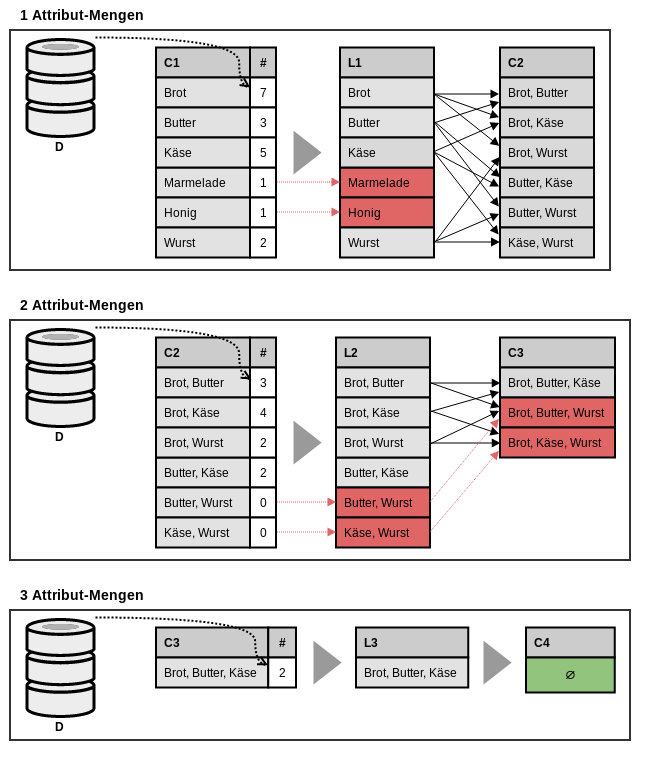
\includegraphics[width=0.8\textwidth]{images/Apriori-Algorithmus.png}
	\caption{Visualisierung des Apriori Algorithmus}
	\source{\cite{association_rule_learning_2017-01-05}}
	\label{fig:konzept:vorgehensweise:apriorialgorithmus}
\end{figure}

$D$ wird benötigt um die Vorkommen zu zählen. Die roten Elemente in $L_k$ werden entfernt weil $minsup$ nicht erreicht wurde, welches im Beispiel den Wert 2 hat. Nach der säuberung von $L_k$ erstellt der apriori\_gen die Kandidaten $C_k$ für den nächsten durchlauf (join). Anschliessend werden in $C_k$ diejenigen Elemente entfernt, welche in $L_{k-1}$ als nicht häufig erkannt wurde (prune). Zum Beispiel kann in $C_3$ das Element {Brot, Butter, Wurst} entfernt werden, da in $L_2$ {Butter, Wurst} den Wert $minsup$ unterschreitet.

Der Algorithmus wird gestoppt, wenn es keine häufigen Kandidaten mehr gibt, was in $C_4$ der Fall ist.

Der Algorithmus kann somit in drei Schritte aufgeteilt werden.
\begin{enumerate}
\item Häufigkeitszählung
\item Generierung der x+1-Attributmenge (Apriori-gen Funktion, join step)
\item Entfernung der Elemente welche den $minsup$ nicht erfüllen (Apriori-gen Funktion, prune step)
\end{enumerate}

Die nachfolgende Apriori-Methode führt die Häufigkeitszählung durch.
Gegen ist die gesamte Datenmenge $D$, welche für die Häufigkeitszählung verwendet wird, sowie der minimum Support welche die Attribute zu erfüllen haben.
\begin{lstlisting}
procedure apriori($D$: Datenmenge; $minsup$: Minimum support) {
	$L_1 \gets$ find_frequent_1-itemsets($D$)
	$k \gets 2$
	while $L_{k-1} \neq \emptyset$ {
		$C_k \gets$ apriori_gen($L_{k-1}$)
		foreach transaction $I \in D$ {
			$C_I \gets \{ c | c \in C_k \wedge c \subseteq I \}$
			foreach candidate $c \in C_I$ {
				count[$c$] $\gets$ count[$c$] + 1
			}
		}
		$L_k \gets \{c | c \in C_k \wedge$ count[$c$] $\ge minsup \}$
		$k \gets k + 1$
	}
	return $\bigcup\limits_{k} L_{k}$
}
\end{lstlisting}
Im ersten Schritt wird die 1-Attributmenge mit häufigen Elementen definiert. In den Zeilen 3 bis 14 wird für $k > 2$ die Items gesammelt, welche öfters vorkommen als der $minsup$. Dazu wird mittels der apriori\_gen Funktion die \textit{Candidates} $C_k$ generiert (Zeile 5).
Anschliessend werden die vorkommen von allen Elementen in $D$ gezählt, wie oft sie in $C_k$ vorkommen (Zeilen 6-12).


\begin{lstlisting}
procedure apriori_gen($L_{k-1}$:frequent (k-1)-itemsets) {
	$C_k \gets \emptyset$
	foreach itemset $l_1 \in L_{k-1}$ {
		foreach itemset $l_2 \in L_{k-1}$ {
			$c \gets \{l_1 \cup \{i\} | i \in l_2 \wedge l_1 \cup \{i\} \notin C_k \}$
			$c_{pruned} \gets c - \{ c' | c' \in c \wedge i \subset c \wedge |i| = k-1 \wedge i \notin L_{k-1} \}$
			$C_k \gets C_k \cup c_{pruned}$
		}
	}
	return $C_k$
}
\end{lstlisting}
In der apriori\_gen Funktion werden k-Attributmengen generiert, indem eine (k-1)-Attributmenge erweitert wird. Dazu gibt es zwei Schleifen welche durchlaufen werden. Auf Zeile 5 wird $l_1$ um Elemente von $l_2$ erweitert. Zudem wird sichergestellt, dass gleiche Mengen nicht mehrfach in $C_k$ hinzugefügt werden können.

Auf Zeile 6 werden die k-Attributmengen gesäubert (prune), indem die neuen Kandidaten $c$ überprüft werden, ob eine Submenge $i$ eines Kandidaten $c'$ nicht in $L_{k-1}$ vorhanden ist. Wenn dies der Fall ist erfüllt $i$ den $minsup$ womit $c'$ den mindest support auch nicht erfüllen kann. Somit kann $c'$ aus $c$ entfernt werden.

% Longer version of apriori_gen
%$c \gets \{l_1 \cup \{i\} | i \in l_2 \wedge l_1 \cup \{i\} \in C_k \}$
%$c_{pruned} \gets \{ i | i \in c \wedge \forall j(j \subset i \wedge |j| = k-1 \wedge j \in L_{k-1}) \}$
%$C_k \gets C_k \cup c_{pruned}$
%
% Looped version of apriori_gen
%	$C_k \gets \emptyset$
%	foreach itemset $l_1 \in L_{k-1}$ {
%		foreach itemset $l_2 \in L_{k-1}$ {
%			if (($l_1$[1] = $l_2$[1]) $\wedge$ ($l_1$[2] = $l_2$[2]) $\wedge$ ... $\wedge$ ($l_1$[$k$-2] = $l_2$[$k$-2]) $\wedge$ ($l_1$[$k$-1] $<$ $l_2$[$k$-1])) {
%				$c \gets l_1 \cup l_2$
%				if not has_infrequent_subset($c, L_{k-1}$) {
%					delete $c$
%				} else {
%					$C_k \gets C_k \cup c$
%					add $C_k \cup c$ 
%				}
%			}
%		}
%	}
%	return $C_k$
%
%
%\begin{lstlisting}
%procedure has_infrequent_subset($c$: candidate k-itemset; $L_{k-1}$: frequent (k-1)-itemsets) {
%	foreach (k-1)-subset $s of c$ {
%		if $s \notin L_{k-1}$ {
%			return TRUE
%		}
%	}
%	return FALSE
%}
%\end{lstlisting}

\subsection{Cluster analysis}
